\section{RNN}
	\begin{figure}[htbp]
		\centering
		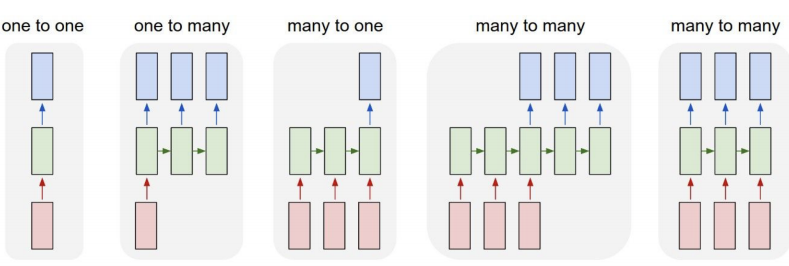
\includegraphics[scale=0.65]{figures/rnn-seqdata.png}
		\caption{各种输入输出方式}
		\label{}
	\end{figure}
	我们之前的网络,都是one-to-one,一个输入,一个输出.
	
	one-to-many:例如看图说话. image->sequence of words
	
	many-to-one.例如动作预测.
	
	many-to-many.例如video captioning.
	
	此外还有offline和online的处理.前者全部看完,后者边看边输出.
	
	Recurrent Neural Network.
	
	\begin{equation}
		\begin{cases}
			h_t = f_W\xk{h_{t-1}, x_t}
			\\
			y_t = f_{W_{hy}}\xk{h_t}
		\end{cases}
	\end{equation}

	Vanilla RNN:
	\begin{equation}
		\begin{cases}
			h_t = \tanh\xk{W_{hh}h_{t-1} + W_{xh}x_t}
			\\
			y_t = W_{hy}h_t
		\end{cases}
	\end{equation}

	计算图,各个方向流向W.
	
	\subsection{Characer-Level Language Model}
	sample:greedy? weighted sampling,根据字母的权,但可能选到冷僻的,比如hh.?更高级:beam search.每次选三个,两层三叉树,选取最后的top3?
	
	实际上将h和x结合的时候,常常先将x进行embedding, W[h,x]->W[h, g(x)].比如,hidden layer可能之后512维,但是输入如果是词向量,那么可能有几万维,非常不均衡.因此将embedding到合适的维度.此外,word embedding已经有现成的处理.
	
	BP时,不同位置的W被loss调用了不同次.这个操作开销极大.
	
	解决方法:truncated BP.截断.比如FP时是从0到t,BP只算从t到t-6.
	
	pytorch的命令:stop\_gradient.

	RNN在长程记忆里会出现问题.delta t一般被称为sequence length.如果过短则相关性不强,过长则cost过多.
	
	RNN tradeoff.
	
	multilayer:2层即可
	
	\subsection{Vanilla RNN Gradient Flow}
	
	tanh的梯度恒小于1,梯度消失.
	
	gradient clipping.
	
	\subsection{LSTM}
	信息传递的一部分放入c?
	
	cell state是long-term memory.我们知道对于普通的tanh,往01之间映射,那么$h_t$和很早之前的$h_i$之间的联系就比较微弱了.而LSTM中的c则一直把信息保留(f也是经过sigmoid激活的,在01之间,可以选择记住或者遗忘),最后h将c进行处理.
	
	核心结构:old info和new info的加和.若f=1,则就是skiplink.换言之c之间有梯度的旁路.
